\chapter{恩格尔曲线与需求曲线}
\label{sec:engel-curve-and-demand-curve}

\section{收入提供曲线与恩格尔曲线}
\index{Engel\rq{}s curve 恩格尔曲线}恩格尔曲线表示消费者在每一收入水平下,对某种商品的消费量。

\begin{equation}
q_1 = f(\overline p_1, \overline p_2, m)
\end{equation}

\begin{figure}[!h]
\colorbox{black!3}{\parbox{\linewidth-2\fboxsep}{%
\centering
\begin{subfigure}[b]{0.5\textwidth}
\centering
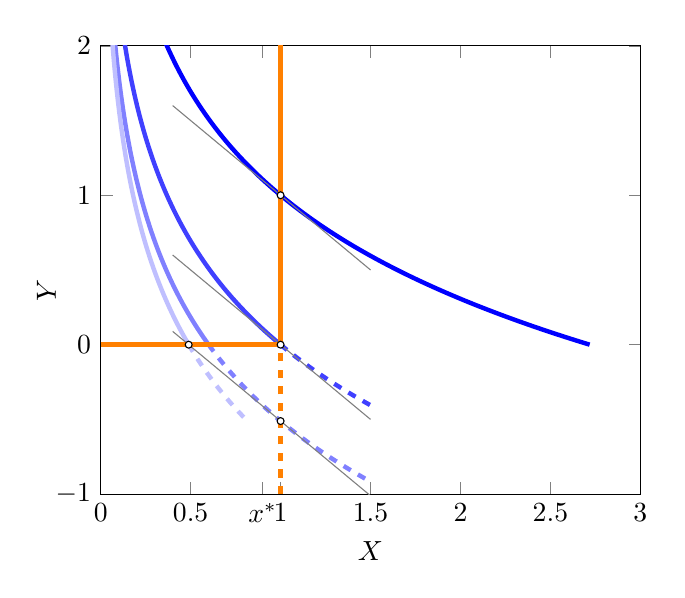
\begin{tikzpicture}
\begin{axis}[
	axis on top=false,
	xmin=0,xmax=3,ymin=-1,ymax=2,
	xlabel style={below},xlabel=$X$,
	ylabel style={left},ylabel=$Y$,
	extra x ticks={0.9},
	extra x tick labels={{$x^*$}},
	samples=200]
\addplot[draw=blue,domain=0:2.718,ultra thick] {1-ln(x)};
\addplot[domain=0:1,draw=blue!75,ultra thick] {-ln(x)};
\addplot[domain=1:1.5,draw=blue!75,dashed,ultra thick] {-ln(x)};
\addplot[draw=blue!50,domain=0:0.6,ultra thick] {-0.511-ln(x)};
\addplot[draw=blue!50,domain=0.6:1.5,dashed,ultra thick] {-0.511-ln(x)};
\addplot[draw=blue!25,domain=0:0.489,ultra thick] {-0.715-ln(x)};
\addplot[draw=blue!25,domain=0.489:0.8,ultra thick,dashed] {-0.715-ln(x)};
\addplot[gray,domain=0.4:1.5] {2-x};
\addplot[gray,domain=0.4:1.5] {1-x};
\addplot[gray,domain=0.4:1.5] {0.489-x};
\addplot[draw=orange,ultra thick] coordinates {(0,0) (1,0) (1,3)};
\addplot[draw=orange,dashed,ultra thick] coordinates {(1,-3) (1,0)};
\addplot[only marks,forget plot,black,mark options={mark size=1.25pt,fill=white},mark=*] coordinates {
	(1,1)
	(1,0)
	(1,-0.511)
	(0.489,0)
	};
\end{axis}
\end{tikzpicture}
\vspace{1.5ex}
\caption{收入提供曲线}
\label{fig:quasilinear-utility-ioc}%
\end{subfigure}%
\begin{subfigure}[b]{0.5\textwidth}
\centering
\begin{tikzpicture}
\begin{axis}[
	domain=0:3,
	xmin=0,xmax=3,ymin=0,ymax=3,
	xtick=\empty,	ytick=\empty,
	xticklabel=\ ,	yticklabel=\ ,
	xlabel style={below},xlabel=$X$,
	ylabel style={left},ylabel=$I$,
	extra x ticks={1},
	extra x tick labels={{$x^*$}},
	samples=300]
\addplot[draw=green,ultra thick] coordinates {(0,0) (1,1) (1,3)};
\addplot[draw=green,ultra thick,dashed] coordinates {(1,0) (1,1)};
\end{axis}
\end{tikzpicture}
\vspace{-1.5ex}
\caption{恩格尔曲线}
\label{fig:quasilinear-utility-engel-curve}%
\end{subfigure}
\caption{拟线性曲线的收入提供曲线和恩格尔曲线}
\caption*{拟线性曲线的特征:整个曲线族可以通过对其中任一条曲线在$y$方向平移得到,见图(\ref{fig:quasilinear-function})。故而对于任意给定的$x$所有曲线上对应的点的切线是等斜率的,其“扩展线”为平行于$y$轴的直线,其收入提供曲线是一条$\righthalfcup$型的折线。}%
\label{fig:quasilinear-utility-and-ioc}%%
}}
\end{figure}

在第\pageref{sec:elastics}页第\ref{sec:elastics}节《弹性》中已经对需求收入弹性的概念做了介绍,在那里无非是为了满足“拓展弹性的应用价值”这个教学目的,一种商品的需求数量和收入水平有怎样的关系都是模糊的。

\subsection{位似偏好的需求的收入弹性为1\footnote{%
格拉韦尔, 里斯. 微观经济学 [M]. 第3版. 上海: 上海财经大学出版社, 2009: 63--64.}}



\subsection{推导收入提供曲线}

注意:通过收入扩展曲线可以得到恩格尔曲线,但收入提供曲线不是恩格尔曲线,有的朋友总说这二者没有差别啊——他们根本不是描述相同变量的相同函数、绘制在不同的坐标系中,怎么会等同呢。


\section{价格消费曲线与需求曲线}

\begin{equation}
q_1 = f(p_1, \overline p_2, \overline m)
\end{equation}


\subsection{推导价格消费曲线}

\section*{推荐阅读}
\markright{推荐阅读}
\addcontentsline{toc}{section}{\hspace{-2.5em}推荐阅读}